\chapter{Advanced Topics \& Quality Assurance with R Markdown} 
\label{sec:practicum4}

\textbf{Learning objectives:} Understand how to write self-documenting makefiles in an organized directory structure, use macros, and write quality assurance reports using R markdown.


\section{Creating a \maken{} help system}
It is sometimes useful to know what a makefile does without having to look through the entire makefile itself. One way of getting that information at a glance is to create a \maken{} help system that prints out the targets and a short summary explaining what each target does. 

To go about creating this help system, you need to create a separate ``help'' makefile that tells \maken{} what to do when you call for help. Before we expand on that, however, let us take a look at the main makefile in the \texttt{testsubject} directory copied over from \texttt{/project_space/}.
\bashcmd{cd ~/testsubject/test001}

Let the variable \$(PROJECT_HOME) represent the pathway to your \texttt{testsubject} directory. You can set this variable in top-level makefile.
\begin{lstlisting}
	PROJECT_HOME=/yourhomedirectory/testsubject
\end{lstlisting}
%\makecmd{PROJECT_HOME=/yourhomedirectory/testsubject}

Open up \texttt{Makefile} in an editor. You will notice that one of first few lines at the top of the file asks \maken{} to include a makefile called \texttt{help_system.mk}; this is the ``help'' makefile that we alluded to earlier. The \texttt{include} directive tells \maken{} to read other makefiles before continuing with the execution of other things in the current makefile.    

As you scroll down, you will see that some of the targets are followed by a \texttt{call} command before their dependencies. For instance, look at the line:
\begin{lstlisting}
	robex: $(call print-help,robex,Alternate skull stripping with ROBEX) T1.nii.gz
\end{lstlisting}
%\makecmd{robex: \$(call print-help,robex,Alternate skull stripping with ROBEX) T1.nii.gz}

This tells \maken{} to return the target \texttt{robex} along with its description when \texttt{print-help} is called (\texttt{print-help} is defined in \texttt{help_system.mk}, as we will see later). Other targets such as \texttt{freesurferskstrip} and \texttt{etiv} also make calls to \texttt{print-help}.

Now, have a look at \texttt{\$(PROJECT_HOME)/lib/makefiles/help_system.mk}.
\begin{lstlisting}
	help: ; @echo $(if $(need-help),,Type `$(MAKE)$(dash-f) help` to get help)
\end{lstlisting}
%\makecmd{help: ; @echo \$(if \$(need-help),,Type \`{}\$(MAKE)\$(dash-f) help\'{} to get help)} % what is happening here?

This line tells \maken{} to echo the fellowing when you type \maken{} into the command line.
\begin{bash}{\maken{}'s Help System}{}
\$ make \\
Type `\maken{} help' to get help
\end{bash}

The variable \texttt{need-help} is set such that \maken{} will filter for the word \texttt{help} in your command line entry to decide whether or not you need help. If so, the function \texttt{print-help} will be called, and this will result in \maken{} printing the name of your targets and their descriptions to your shell. Depending on whether or not this will be helpful for you, you may want to copy \texttt{help_system.mk} to your own project directory and include it in your top-level Makefile. 

We will not reproduce the details of how \texttt{help\_system.mk} works in this practical. For an excellent description of this simple but useful system, please refer to page 181 of John Graham-Cumming's GNU Make Book, or to his \href{http://www.cmcrossroads.com/article/self-documenting-makefiles}{blog posting}.  

\section{Makefile Directory Structure}
Often several people collaborate to work on analyzing different types of data from a project and this calls for several makefiles. Or, you may wish to split up a processing pipeline into various parts as we have in our Makefile example. In the main makefile \texttt{Makefile} from the \texttt{\$(PROJECT\_HOME)/test001} directory -- and this was mentioned earlier -- you should have noticed that several other makefiles were included. 

\begin{lstlisting}
	include $(PROJECT_HOME)/lib/makefiles/help_system.mk \\
	include $(PROJECT_HOME)/lib/makefiles/resting.mk \\
	include $(PROJECT_HOME)/lib/makefiles/xfm.mk \\
	include $(PROJECT_HOME)/lib/makefiles/fcconnectivity.mk \\
	include $(PROJECT_HOME)/lib/makefiles/QA.mk 
\end{lstlisting}

%\makecmd{
%include \$(PROJECT_HOME)/lib/makefiles/help_system.mk \\
%include \$(PROJECT_HOME)/lib/makefiles/resting.mk \\
%include \$(PROJECT_HOME)/lib/makefiles/xfm.mk \\
%include \$(PROJECT_HOME)/lib/makefiles/fcconnectivity.mk \\
%include \$(PROJECT_HOME)/lib/makefiles/QA.mk 
%}

Here, we see that there are makefiles for:
\begin{easylist}[enumerate]
	& defining the \maken{} help system.
	& processing resting-state data called \texttt{resting.mk} (this is documented in detail in \nameref{example:restingstate}).
	& obtaining transformation matrices for registrations called \texttt{xfm.mk} (see \nameref{example:testsubjectxfm} for documentation).
	& running seed-based connectivity analysis called \texttt{fcconnectivity.mk} (see \nameref{example:fcconnectivity} for documentation).
	& creating QA reports called \texttt{QA.mk} (see \nameref{example:testsubjectQA} for documentation).
\end{easylist} 

For a full description of the makefiles (excluding \texttt{help\_system.mk}), we encourage you to refer to their full documentation. 

Note that makefiles should be stored in the \texttt{lib} directory as we did in this example. This is good practice and helps keep your directories organized and less cluttered. The importance of creating a tidy directory tree structure has been continually emphasized throughout this course. Refer to \hyperref[sec:practicum3]{Practical 3} or \hyperref[sec:dir]{Chapter 2} of the manual for a more thorough discussion of the directory structure common to most IBIC projects.

\section{The \texttt{clean} target}
In \maken{}, the \texttt{clean} target normally delete all unnecessary files that were created in the process of running \maken{}. Remember that storage is limited on IBIC systems! Cleaning up your project directory will make space for future projects that you will be working on. The target itself is usually specified last in a typical \maken{} recipe, and must be included in your list of \texttt{.PHONY} targets if you choose to define it. 

Now, go to your \texttt{\$(PROJECT\_HOME)/test001/} directory and open \texttt{Makefile} in an editor. Scroll all the way down. You will see both an \texttt{archive} and \texttt{clean} target. \texttt{archive} is a target intended to clean up the directory for archiving after a paper has been accepted. The purpose of this target is to retain important results but remove the partial products. Obviously, what you define as ``important results'' depend upon the kind of analysis that you are doing and the amount of risk you are willing to assume.

The \texttt{clean} target in this makefile includes \texttt{clean\_qa} and \texttt{clean\_rest} which are themselves targets in other makefiles in the \texttt{lib/} directory. Typically, files that are ``easy'' to make and are no longer necessary can be removed. Other files, such as those generated by FreeSurfer's \texttt{recon-all}, require more compute resources and are not as easily remade. Other examples of files that you may not want to remove include hand-edited files, and end stage products of quantitative processing pipelines. You should therefore think carefully about what you want to remove and what you want to keep. 

\section{Creating New Makefile Rules On The Fly}
One of the drawbacks of implicit rules in \maken{} is that they can only substitute one pattern at a time. For example, we may give multiple fMRI task blocks (which could be matched by one pattern) but then wish to process each contrast of parameter estimates (COPE) using an implicit rule. Thankfully, there is a way to ``create new makefile rules on the fly'' using functions built in to \maken{}. We will work through an example that overrides default Feat registration and does just this (see \nameref{section:antsreg}).


\section{Incorporating R Markdown into \maken{}}

Quality assurance (QA) is an important step in a neuroimaging analyses pipeline. At IBIC, data is typically preprocessed and checked for quality before proceeding with further analyses. This can be done both qualitatively and quantitatively. Some of the common aspects of data that are looked at include motion outliers, quality of brain registration/normalization to a subjects-specific or standard template, and whether brain segmentation has been performed correctly. 

While neuroimaging packages usually include QA tools of their own (such as FSL's FEAT report), built-in QA tools have limited application when you are using more than one neuroimaging package to process your data or if you want to view your data in a non-traditional way. 

Know that you may certainly create QA measures for each subject in your project and inspect these one-by-one or examine NIfTI images created at various stages with a previewer, but this may be inconvenient and time-consuming. Because there usually are several things that have to be inspected during a quality assurance procedure, it is incredibly helpful to have images and data parameters or statistics displayed on a single page for each subject in a project. Alternatively, you may choose to look at a single aspect of your data and would like to concatenate a QA measure from all of your subjects into one report. This is where R Markdown comes in.

R Markdown is an authoring format that allows us to generate reports using a simple markup language (\url{http://rmarkdown.rstudio.com}). It is extremely versatile in that it can incorporate code from multiple languages (including HTML, \bashn{}, \texttt{python} and \texttt{R}) to generate HTML and PDF documents, or even interactive web applications. 

Although QA reports be viewed using PDF documents or HTML pages, at IBIC we prefer to use the HTML format for a couple of reasons. For one, a HTML report gives us the ability to look at moving GIF images, which are useful when we want to view the collected brain scans as a time series. In addition, it circumvents the issue of pagination and allows us scroll seamlessly through all our images and statistics in a single page. PDFs, tend to be more cumbersome to use as images may be awkwardly split between pages and cause page breaks if they are not properly sized.

Go to the directory \texttt{\$(PROJECT\_HOME)/freesurfer/QA} and open up \texttt{QA\_check.html} with your internet browser. 
\bashcmd{iceweasel QA\_check.html}

Clicking on the link \texttt{testsubject} will redirect you to a page that holds the images generated by FreeSurfer. Here, you can see the segmented and parcellated brain of the subject, along with images showing the surface curvature of the brain. This page is automatically created by FreeSurfer's recon-all.

We can also create our own QA images to, say, check whether a T1 brain has been properly registered to a brain in standard space. These images can be specified as targets in your makefile as follows.
\begin{lstlisting} 
	QA/images/T1_to_mni_deformed.png: xfm_dir/T1_to_mni_deformed.nii.gz $(FSLpath)/data/standard/MNI152_T1_2mm_brain.nii.gz 
		mkdir -p QA/images ;\
		$(FSLpath)/bin/slicer $(word 1,$^) $(word 2,$^) -s 2 -x 0.35 sla.png -y 0.35 slb.png -z 0.35 slc.png ;\
		pngappend sla.png + slb.png + slc.png QA/images/intermediate1.png ;\
		$(FSLpath)/bin/slicer $(word 2,$^) $(word 1,$^) -s 2 -x 0.35 sld.png -y 0.35 sle.png -z 0.35 slf.png ;\ 
		pngappend sld.png + sle.png + slf.png QA/images/intermediate2.png ;\ 
		pngappend QA/images/intermediate1.png - QA/images/intermediate2.png $@ ;\ 
		rm -f sl?.png QA/images/intermediate?.png
\end{lstlisting}

Here, FSL \texttt{slicer} is used to create 2D images from 3D images. To get a better understanding of how slicer is used, simply type \texttt{slicer} into the command line. \href{http://fsl.fmrib.ox.ac.uk/fsl/fslwiki/Miscvis}{This FSL page} also provides a brief description of what slicer does. 

In the context of the above example, \texttt{slicer} first overlays the \texttt{T1_to_mni_deformed} image on top of the MNI152 brain. Subsequently, it creates several 2D images named \texttt{sl?.png} that come from sagittal, coronal or axial slices. This is indicated by the \texttt{-x/y/z} flags used followed by the name of the image generated. Note that these files are temporary! Once \texttt{pngappend} has been used to paste these images next to each other to generate a single image, the temporary files are removed. If you are using FSL \texttt{slicer} for more than one instance in a makefile, the temporary files created may cause \maken{} to crash if they are given the same names and are put into the same directory when \maken{} is run in parallel. Make sure that the names of your outputs from FSL slicer do not overlap each other. 

Given that the code used to generate QA images can be very messy and ugly, you may want to create a \bashn{} script to create those images and call that from your QA makefile instead. This also avoids potential problems that may arise when many similarly named temporary files are generated that may cause \maken{} to continually overwrite these files when using a tool like FSL \texttt{slicer} in parallel. A wonderful example of such a script can be found at \texttt{\$MAKEPIPELINES/tapping/bin/sliceappend.sh} (credit goes to Matt Peverill!). 

Once we have created all the QA images we want to include in our HTML report, we need to create a \texttt{.Rmd} file that tells R Markdown where to find these images. 

Now let us have a look at a subsection of a \texttt{.Rmd} file on the next page. The file is \texttt{\$(PROJECT\_HOME)/lib/Rmd/fMRI.Rmd}. 

\begin{bash}{Example of a R Markdown File}{}

--- \\
title: Quality Assurance of Preprocessing for TASK for ID SUBJECT \\
output: \\
  html\_document: \\
    keep\_md: no \\
    toc: yes \\
    force\_captions: TRUE \\
--- \\
\#T1 Skull-Strip \\

<img src=``/project\_space/makepipelines/testsubject/test001/QA/images/T1\_skstrip.gif'' width=``500px'' /> \\

\#Parameters \\

\#\#Time Series Difference Analysis \\

<img src=``/project\_space/makepipelines/testsubject/test001/QA/images/TASK\_tsdiffana.gif'' width=``750px'' /> \\

\# MOTION \\

\#\#Motion Statistics \\

\`{}\`{}\`{}\{r engine='bash', echo=FALSE\} \\
val=\`{}cat /project\_space/makepipelines/testsubject/test001/rest\_dir/TASK\_mean\_abs\_disp.txt\`{} \\
echo ``Mean Absolute Displacement : \$val mm'' \\
val=\`{}cat /project\_space/makepipelines/testsubject/test001/rest\_dir/TASK\_mean\_rel\_disp.txt\`{} \\
echo ``Mean Relative Displacement : \$val mm'' \\
\`{}\`{}\`{} \\

\end{bash}

A \texttt{.Rmd} file should always begin with a demarcated section listing the title of the report and the type of file to be created. We see that the output here is a HTML document. \texttt{toc} refers to table of contents. %\texttt{force_captions} allows you to specify the dimensions of an image in html text (????). % Can't find any documentation explaining what force_captions does 

In R Markdown, the size of headers depend on the number of \mypound (hash) symbols used before the name of a header. This is akin to how the titles of major sections of a text are rendered in the largest text size, and subsections along with sub-subsections are printed in smaller-size text. A double hash symbol before a title will mean that the title will be treated as a ``sub-section'' and be printed in smaller size than the main headers. As the number of hash symbols used before a title increases, the text becomes smaller.

Notice that HTML syntax is used to insert images into the report. Heights and widths of images can be specified as well. 

Assuming we want to print out some information about the subject into the report, we can use \bashn{} within a R Markdown file to \texttt{grep} for the stuff we need or \texttt{cat} a value from a file. In the example above, we open the bash script portion of the file with three backticks and a curly bracket telling R that the following text is written in \bashn{} code. Here, we are asking \bashn{} to \texttt{cat} the values from two text files that gives us the mean absolute and mean relative displacement in mm (see \texttt{cat} help if you are not familiar with its usage). These will then be printed out into our HTML report.

Once we have a \texttt{.Rmd} file ready, we want to tell \maken{} to create the HTML report for us. By doing so, we can parallelize the generation of QA reports. We do this by inserting a target such as the following into our QA makefile (which is fully documented in \nameref{example:testsubjectQA}):

\begin{lstlisting}
	QA/rest_Preprocessing.html:  (PROJECT_HOME)/lib/R/fMRI.Rmd TSNR MotionGraphs SkullstripQA
		sed -e `s/SUBJECT/$(subject)/g' -e `s/TASK/rest/g'  $(word 1,$^) > QA/rest_Preprocessing.Rmd ;\
		R -e `library(``rmarkdown'');rmarkdown::render(``QA/rest_Preprocessing.Rmd'')' 
\end{lstlisting}

The target is your HTML file, and the dependencies are your \texttt{.Rmd} file and your images or whatever else you decide to include in your report. The output is dependent on the \texttt{.Rmd} file to trigger to regenerate when the source has been changed. We then use \texttt{sed} to replace instances of the string ``SUBJECT'' in the R Markdown file with the actual subject ID. The subject ID variable \texttt{\$subject} should have been set at the initial portion of your makefile. 

\maken{} will then call R to load the package ``rmarkdown'' so that it can read R Markdown, and proceed to generate/render your report, which will look something like \autoref{fig:qareport}. 

\begin{figure}
	\begin{center}
		\includegraphics[scale=.6]{../images/QAcropped.eps}
		\caption{QA report in R Markdown}
		                \label{fig:qareport}
	\end{center}
\end{figure}

Holy Bad Skullstripping! This is one of the many reasons why we do QA. The full report can be viewed in your favorite Internet browser and can be found at \texttt{\$(PROJECT\_HOME)/test001/QA/rest\_Preprocessing\_example.html}. 
 
And that's it! 





